\documentclass[11pt]{article}
\usepackage[T1]{fontenc}
\usepackage{lmodern,microtype}
\usepackage[margin=1in]{geometry}
\usepackage{amsmath,amssymb,amsthm,mathtools}
\usepackage{booktabs,longtable,array,enumitem}
\usepackage{tikz}
\usetikzlibrary{positioning,arrows.meta}
\usepackage{xurl}
\usepackage[colorlinks=true,linkcolor=blue!45!black,citecolor=blue!45!black,urlcolor=blue!45!black]{hyperref}
\hypersetup{pdftitle={Polynomial Marked-Cut Kernels for Arbitrary Disconnected Tile Powers},pdfauthor={Research continuation prepared for the ProveIt project},pdfsubject={Stable seam decomposition and compressed unknot-hierarchy terminal graphs}}
\usepackage{fancyhdr}
\pagestyle{fancy}\fancyhf{}\fancyhead[L]{\small Disconnected tile kernels}\fancyhead[R]{\small ProveIt research continuation}\fancyfoot[C]{\thepage}
\setlength{\headheight}{14pt}
\newtheorem{theorem}{Theorem}[section]
\newtheorem{lemma}[theorem]{Lemma}
\newtheorem{proposition}[theorem]{Proposition}
\newtheorem{corollary}[theorem]{Corollary}
\newtheorem{definition}[theorem]{Definition}
\theoremstyle{remark}\newtheorem{remark}[theorem]{Remark}
\newcommand{\Sig}{\mathsf S}
\newcommand{\rk}{\operatorname{rk}}
\newcommand{\poly}{\operatorname{poly}}
\newcommand{\bits}{\operatorname{bits}}
\newcommand{\lcm}{\operatorname{lcm}}
\newcommand{\size}[1]{\lVert #1\rVert}
\DeclareRobustCommand{\code}[1]{\nolinkurl{#1}}
\title{\textbf{Polynomial Marked-Cut Kernels\\for Arbitrary Disconnected Tile Powers}\\[6pt]
\large Stable seam decomposition, cyclewise compression,\\and a bounded-depth route for unknot-hierarchy terminals}
\author{Research continuation prepared for the ProveIt project\\\small Prepared with ChatGPT; proofs and implementation supplied for review}
\date{12 October 2026}
\begin{document}
\maketitle
\begin{abstract}
The preceding four-copy report proves that the threshold-three marked cut signature of a connected graph tile stabilizes after four serial copies. Disconnected tiles exhibit genuine permutation effects, and its extension through a common permutation period need not give a polynomial-size kernel. We remove the connectedness restriction without expanding that common period.

For any finite undirected multigraph tile of width $w$, any positive binary exponent $N$, and any fixed cut threshold $k$, we construct a graph with the same complete marked boundary-cut signature and $O((k+3)(w+1)^2\size{T})$ vertices and edges. Construction is polynomial in the encoded input. The argument first obtains a rank-stable power after at most $w+1$ copies, then separates its seams into through channels, one-sided attachments, and detached pieces. Each through channel follows its own component cycle. Only that cycle's length, at most $w$, enters its connected repetition reduction. Loops, parallel edges, isolated vertices, dying channels, component mergers, and exact absence of either edge mark are retained.

We also prove a polynomial transient bound for eventual periodicity, a contextual replacement theorem, binary source-coloring lifting, and compositional bounds for nested assembly expressions. In particular, fixed-threshold graph queries on logarithmic-depth, polynomial-width descriptions admit quasi-polynomial bounds. This is a theorem about a specified graph-description class, not an unrestricted unknot-recognition theorem.

The standard-library implementation passes 37 tests, 6,000 complete signature comparisons, all 4,360 boundary partitions through width four, 1,800 literal source-cell-cover audits, 700 cubic-source checks, and 250 nested-expression comparisons. Paired graph-query/replay measurements include both gains and regressions. A native source-pattern exporter, a fully independent compression verifier, and the complete hierarchy complexity bound are not delivered here.
\end{abstract}
\vfill
\noindent\textbf{Source checkpoint.} Targeted repository inspection is pinned to
\code{ed166080d7db14dd7a91d07788996f02947dd92a}. No repository write or upstream integration was performed.
\clearpage
\setcounter{tocdepth}{1}
\tableofcontents
\clearpage

\section{Research position and the concrete advance}
\subsection{What the repository already supplies}
The maintained raw-cut construction stores all cell dimensions and their source attaching charts in binary affine families. Its later source-parallelity construction includes product handles of indices zero, one, and two, together with complete base polygons and fibre information. The inherited complementary core has at most $30T$ handles and at most $66T$ core-facing base arcs for $T$ source tetrahedra \cite{rawcut,parallelity}. These are existing results, not contributions of this article. An inherited source core is not yet an admissible patterned hierarchy structure.

The recent incoming four-copy report addresses a subsequent operation: testing the essentiality of a large boundary graph pattern on a separately certified ball. It gives a width-independent kernel for flat repetitions of \emph{connected} tiles. It also exhibits a disconnected swap tile whose zero-cost boundary relation depends on parity. Its restricted disconnected extension uses a common permutation order $h$, and explicitly leaves more general zero-cost connectivity relations as a research question \cite{fourcopy}.

This continuation resolves that question for finite serial graph tiles with distinct input and output ports. The new reduction is polynomial in width, rather than independent of width. Its important improvement is the removal of both numerical multiplicity and the potentially large common period from the explicit output size. The scope is every finite tile satisfying the interface contract, not just one selected family of permutations.

\subsection{The topological role and its boundary}
In Lackenby's hierarchy algorithm, a terminal component is a ball with an essential boundary pattern; the graph criterion is not a ball-recognition algorithm. The July 2026 manuscript separately discusses the number of hierarchy steps and the need to specify operation costs \cite{lackenby2026}. We improve one possible representation-dependent terminal cost. We do not infer a short geometric hierarchy from a short graph kernel.

Three distinctions will be maintained throughout. First, a query-equivalent graph is not a replacement three-manifold or an isotopic boundary pattern. Second, a source-complete graph descriptor must be exported from the actual transported pattern, not guessed from a normal multiplicity or a list of base-component genera. Third, a quasi-polynomial bound for a bounded-depth description class does not show that every knot produces such a description.

\subsection{Attribution and novelty scope}
The complete four-mark signature, its compositional law, and the sharp connected four-copy theorem are taken from the incoming report \cite{fourcopy}; their short proofs are recalled to make the extension self-contained. Partition monoids and their diagram calculus are established objects \cite{eastgray}. Thresholded cut sparsification is also an established subject: connectivity-threshold mimicking networks preserve terminal cut values in small graphs \cite{mimicking,liu}. Our construction instead preserves two additional \emph{exact} monochromatic-edge marks, works directly on a binary serial power, and explicitly handles its source component structure.

The contribution developed here is the combination of a bounded stable power, a source-edge-preserving seam decomposition, cyclewise connected compression, and its compositional consequences. We do not claim invention of Green-relation methods, cyclic edge connectivity, max-flow certificates, or binary powering. The literature comparison is targeted, not a priority certification for the specialized theorem proved below.

\section{Graphs, interfaces, and exact marked signatures}
\subsection{The input contract}
All graphs are finite undirected multigraphs. Edges are occurrences: parallel edges are not merged, and loops are retained. A loop contributes two to degree. A width-$w$ tile is a graph $T$ with ordered vertex lists
\[
 L=(\ell_1,\ldots,\ell_w),\qquad R=(r_1,\ldots,r_w),\qquad w\ge1,
\]
whose entries are distinct and for which $L\cap R=\varnothing$. A tile may be disconnected and may contain isolated vertices or components meeting no ports. Serial composition takes fresh graphs and identifies $r_i$ of the first with $\ell_i$ of the second. No edge is identified, contracted, or deleted. Write $T^N$ for the $N$-fold serial power; exponents are positive. An exponent-zero identity would have coincident input and output vertices and requires a different interface convention.

For intermediate pieces we allow unequal nonempty input and output widths. They are composed only when adjacent ordered lists have equal length. The connected periods used for capping always have equal widths. Put
\[
 \size{T}=|V(T)|+|E(T)|+2w,\qquad B=\bits(N).
\]
This is a combinatorial size; vertex identifiers, the exponent, and provenance records have their own bit costs.

\subsection{The two edge marks}
For a coloring $c:V(G)\to\{0,1\}$ define
\[
 q_G(c)=\#\{uv\in E(G):c(u)\ne c(v)\},\qquad
 F_G(c)=\{a:\exists uv\in E(G),\ c(u)=c(v)=a\}.
\]
The set $F_G(c)$ is exact. In particular, $F=\varnothing$ forbids \emph{every} monochromatic edge, including loops. A marked cut at threshold $k$ has $q\le k$ and $F=\{0,1\}$.

For boundary colorings $\alpha,\beta\in\{0,1\}^w$ and $F\subseteq\{0,1\}$, let
\begin{equation}\label{eq:signature}
 \Sig_k(G)[\alpha,\beta,F]
 =\min\left(k+1,\min_{\substack{c|_L=\alpha,\ c|_R=\beta\\F_G(c)=F}}q_G(c)\right).
\end{equation}
An empty inner minimum is infinity. Thus $k+1$ means either infeasibility or a cost above the threshold. The four entries indexed by $F$ must not be replaced by an ordinary unmarked cut value.

\begin{lemma}[Compositionality]\label{lem:compose}
If graphs meet only at their named interfaces and their edge sets are fresh, their marked signatures compose by minimum, addition of costs, and union of exact mark sets. In particular,
\[
 \Sig_k(A\circ B)[\alpha,\gamma,F]
 =\min_{\substack{\beta,F_1,F_2\\F_1\cup F_2=F}}
 \min\{k+1,\Sig_k(A)[\alpha,\beta,F_1]+\Sig_k(B)[\beta,\gamma,F_2]\}.
\]
Equality of signatures permits replacement in every external graph context that touches only the named vertices. The context may prescribe colors or impose further identifications among those vertices.
\end{lemma}
\begin{proof}
Compatible colorings on the pieces glue uniquely. Costs add because edge occurrences belong to exactly one piece, and the exact mark set is the union of their marks. Conversely, every global coloring restricts in this way. Nonnegative costs make clipping commute with addition and minimum. The same argument after fixing the context's coloring proves the contextual statement.
\end{proof}
The proof uses exponentially large tables only as a mathematical language. The production constructor never enumerates interface colorings.

\subsection{The inherited connected reduction}
Set
\begin{equation}\label{eq:cutoffs}
 c_k=\begin{cases}4,&k=3,\\k+2,&k\ne3,\end{cases}
 \qquad d_k=\max\{2,k+1\}.
\end{equation}
\begin{lemma}[Connected repetition, recalled from \cite{fourcopy}]\label{lem:connected}
For a connected tile $A$,
\[
 \Sig_k(A^m)=\Sig_k(A^{\min(m,c_k)}).
\]
At threshold three the uniform cutoff four is optimal.
\end{lemma}
\begin{proof}
A zero-cost coloring of a connected tile is monochromatic, has equal constant boundary colors, and contributes its one color mark. A coloring of a long power with cost at most $k$ has at most $k$ positive-cost copies. Keep those and at most one zero-cost copy of each color. This leaves at most $k+2$ copies and preserves endpoints, cost, and exact marks. A retained zero-cost copy permits padding. Conversely, a coloring of $k+2$ copies with cost at most $k$ has a zero-cost copy and can be extended arbitrarily.

For $k=3$, if there are at most two positive-cost copies, the same argument uses at most four copies. If there are three, each costs one. When their union of marks is nonempty, at most one zero-cost copy supplies any missing mark, or can be retained for padding. If all three are markless, every edge of the tile is bichromatic in each of them; cost one forces the connected tile to be a single edge. Three flips have opposite endpoints. If both zero-cost color marks are needed, replace the coloring by a monochromatic first-color edge, one flip, and a monochromatic second-color edge, and pad to four. This may lower the cost of an individual coloring, which is enough for equality of minima. The reverse direction again pads a zero-cost copy.

For optimality, a single-edge tile with both external colors zero needs four edges to have both marks: a zero edge, a one edge, and two flips. Three copies cannot supply these, whereas the path coloring $0,0,1,1,0$ on four edges does.
\end{proof}

\begin{lemma}[Detached repetition]\label{lem:detached}
Let $J$ be any graph with no named ports. Disjoint unions of $m$ copies and of $\min(m,d_k)$ copies have the same clipped minimum for every exact mark set.
\end{lemma}
\begin{proof}
If $J$ has no edges, every coloring has empty marks and zero cost. Otherwise, either singleton mark is realized at cost zero by a monochromatic coloring. With at least two copies, both marks are realized at cost zero by coloring whole copies differently. For empty marks every edge is bichromatic, so any feasible coloring costs exactly $m|E(J)|$. Once $m\ge k+1$ this is above threshold; infeasibility also stays above threshold. Counts below the cutoff are unchanged. This handles disconnected $J$ as well as connected components.
\end{proof}
The exact empty-mark condition explains why detached repeated edges cannot simply be discarded. Keeping two copies alone is insufficient for all thresholds.

\section{A bounded transient in the boundary partition monoid}
\subsection{The partition associated with a tile}
The connected components of $T$ induce a partition $p(T)$ of its $2w$ named ports. Multiplying partitions means gluing the two middle rows of a three-row diagram, taking connectivity, and retaining the two outer rows. Components meeting neither outer row are ignored \emph{only for this connectivity calculation}. The original graph edges will be retained later.

A block is through if it meets both rows, and $\rk(p)$ denotes the number of through blocks. Directly from the diagram,
\[
 p(A\circ B)=p(A)p(B),\qquad \rk(ab)\le\min\{\rk(a),\rk(b)\}.
\]
These statements concern connectivity, not homology or marked cut values.

\begin{lemma}[Rank-preserving right division]\label{lem:division}
If $b=az$ and $\rk(b)=\rk(a)$, there is a partition $x$ with $bx=a$. It can be constructed using $O(w)$ stored port labels and checked by a partition product.
\end{lemma}
\begin{proof}
Every through block of $b$ descends from a through block of $a$. Since the ranks agree, none of the latter dies or merges with another. Their upper vertex sets are therefore unchanged, while upper-only blocks are unaffected by right multiplication.

For each through block of $a$, identify its matching through block of $b$ by this common upper set. Choose one lower vertex of the latter. In $x$, connect that chosen upper vertex to all lower vertices belonging to the desired lower part of the block of $a$. Create the lower-only blocks of $a$ as lower-only blocks of $x$. Leave every other upper vertex of $x$ a singleton. Multiplication by $b$ now reconnects each unchanged upper through block to exactly its prescribed lower set. Unused middle components disappear, and upper-only blocks remain unchanged. Thus $bx=a$.
\end{proof}

\begin{theorem}[A short stable power]\label{thm:stable}
For every width-$w$ boundary partition $p$, there is an $s\le w+1$ such that
\[
 \rk(p^s)=\rk(p^{s+1})=\rk(p^{s+j})\quad(j\ge0).
\]
A certificate consists of $s$, the two consecutive powers, and a partition $x$ satisfying $p^{s+1}x=p^s$. In particular,
\[
 \rk\bigl((p^s)^2\bigr)=\rk(p^s).
\]
\end{theorem}
\begin{proof}
The integer sequence of ranks is nonincreasing and lies between zero and $w$. Among the first $w+1$ comparisons there is an equality, giving some $s\le w+1$. Lemma~\ref{lem:division} gives $p^{s+1}x=p^s$. Multiplying on the left by $p^j$ yields
\[
 p^{s+j+1}x=p^{s+j}.
\]
Rank monotonicity in the two directions forces equality for every $j$. Taking $j=s$ gives the final assertion.
\end{proof}
This is stronger than a doubling argument that allows an exponentially large stable power. The right-division identity is the reason a first plateau cannot be followed by a later rank drop.

\noindent\textbf{A long transient is real.} Take edges $\ell_i r_{i+1}$ for $1\le i<w$, with the two remaining endpoint ports isolated. The ranks of successive powers are $w-1,w-2,\ldots,0,0,\ldots$. Thus a width-linear transient is necessary in general. Conversely, a permutation matching has constant rank from the first power, even when its permutation has large order. Stability of rank is not stabilization of the partition itself.

\section{Stable seams and connected channel pieces}
\subsection{Four kinds of source components}
Let $U=T^s$ be the explicit stable power supplied by Theorem~\ref{thm:stable}. It has size at most $s\size{T}$. Write its connected components as through, input-only, output-only, or internal, according to which port lists they meet. Let $\mathcal H$ be the set of through components, and put $r=|\mathcal H|$.

To analyze a seam between two copies of $U$, construct a finite graph $Z$ as follows. Include the complete output-only components of the left copy and the complete input-only components of the right copy. Include the output port vertices of left through components and the input port vertices of right through components, but \emph{not their other edges or vertices}. Perform all coordinatewise seam identifications. The connected components of this graph are the seam pieces. A direct identification between two through ports is a legitimate zero-edge seam piece.

\begin{lemma}[Stable seam classification]\label{lem:seam}
Every component of $Z$ touches at most one left through component and at most one right through component. The pieces touching both sides determine a permutation
\[
 \pi:\mathcal H\longrightarrow\mathcal H.
\]
Every $H\in\mathcal H$ participates in at least one two-sided seam piece, and all its such pieces meet the same $\pi(H)$.
\end{lemma}
\begin{proof}
If a seam component met two left through components, those two components would merge in $U^2$. At most one through component can arise from each original one, so this would reduce rank. The same argument applies on the right. If a left through component had no route to a right through component, it would die in the product, also reducing rank. In the bipartite incidence graph of seam pieces and through components, a route between left and right must contain a seam piece touching both: all intermediate through vertices, if present, are on one of the two sides, and cannot be distinct on that side without causing a merger. Finally, two different right partners for one left component would merge those right through components. Thus the partner relation is a bijection.
\end{proof}
Notice that a one-sided seam piece is allowed. It may be attached to the main through component without itself meeting the next one. Failing to separate such pieces is one reason a naive ``one source component equals one tile'' rule is incorrect.

\subsection{A deterministic edge-ownership convention}
Classify a seam component as $L$, $R$, $B$, or $F$, according as it touches only a left through component, only a right through component, both, or neither. Assign its edges as follows:
\begin{center}
\begin{tabular}{lll}\toprule
Kind & Owner & Role\\\midrule
$L$ & Left through piece & Outgoing one-sided attachment\\
$R$ & Right through piece & Incoming one-sided attachment\\
$B$ & Left through piece & Bridge to the next through piece\\
$F$ & Separate detached graph & Repeated seam island\\\bottomrule
\end{tabular}
\end{center}
The convention concerns graph-edge ownership, not contraction of those edges. Its asymmetry is intentional: it makes connected pieces with disjoint interfaces.

For $H\in\mathcal H$, define $D_H$ to contain the entire graph $H$, all $R$-pieces on the preceding seam that attach to $H$, and all $L$- and $B$-pieces on the following seam that attach to $H$. Its input vertices are precisely the vertices of $H$ touched by incoming $B$-pieces. Its output vertices are precisely the vertices of the next through component $\pi(H)$ touched by outgoing $B$-pieces. Order both lists by the corresponding original input-port indices of $U$.

\begin{lemma}[Connected decorated pieces]\label{lem:decorated}
Each $D_H$ is connected, has nonempty disjoint input and output lists, and has output list compatible with the input list of $D_{\pi(H)}$. The sum of their combinatorial sizes is $O(\size{U})$.
\end{lemma}
\begin{proof}
The central component $H$ is connected. Every added seam piece meets it, so the union is connected. Lemma~\ref{lem:seam} supplies at least one incoming and outgoing bridge. Incoming vertices lie in the original input list of the central $H$. Outgoing vertices lie in the next copy's through input list; a direct seam identification may identify such a vertex with an original output vertex of $H$, but never with an original input vertex of $H$. Distinct source port lists and pairwise coordinate identifications therefore keep the two lists disjoint.

All bridge pieces from $H$ go to its unique partner. They expose exactly the same ordered set of input vertices that the partner receives. There is no assertion that these lists have the same size for different $H$; only adjacent lists must agree.

Each central through edge is used once. Each edge of an input-only or output-only source component occurs in exactly one seam piece and is assigned once, unless that piece is detached. Nonthrough source vertices are likewise used a bounded number of times; extra exposed through vertices are bounded by the number of port incidences. Summing gives $O(\size{U})$.
\end{proof}

\paragraph{The important interface restriction.}
A bridge component may also contain many vertices of an input-only component. Those are \emph{internal vertices of the bridge}, not ports of the next decorated tile. Only vertices belonging to the partner through component become output ports. This distinction is enforced by the reference implementation and by a dedicated regression case. Including every source input vertex seen in a bridge would add disconnected or inappropriate ports.

\begin{figure}[ht]
\centering
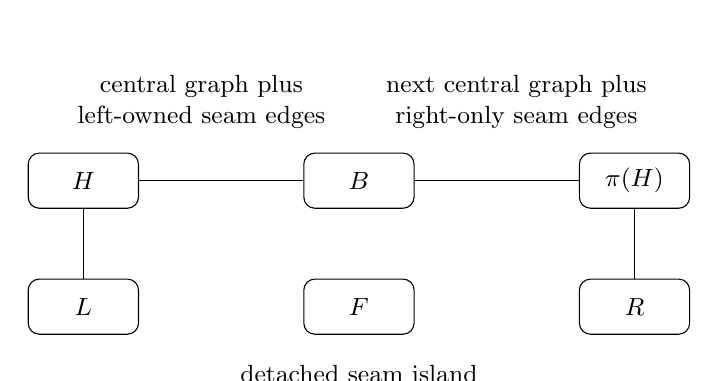
\begin{tikzpicture}[>=Latex, every node/.style={font=\small},box/.style={draw,rounded corners,minimum width=1.4cm,minimum height=.7cm}]
\node[box] (h) at (0,1.2) {$H$};
\node[box] (b) at (3.5,1.2) {$B$};
\node[box] (j) at (7,1.2) {$\pi(H)$};
\node[box] (l) at (0,-.4) {$L$};
\node[box] (rr) at (7,-.4) {$R$};
\node[box] (f) at (3.5,-.4) {$F$};
\draw (h)--(b)--(j);\draw(h)--(l);\draw(j)--(rr);
\node[align=center] at (1.5,2.2) {central graph plus\\left-owned seam edges};
\node[align=center] at (5.5,2.2) {next central graph plus\\right-only seam edges};
\node[align=center] at (3.5,-1.25) {detached seam island};
\end{tikzpicture}
\caption{A component-incidence schematic, not an embedding of a boundary pattern. A seam piece touches at most one through component on each side. Bridge edges are assigned to the left; the actual right-through vertices they meet form the interface.}
\end{figure}

\subsection{Exact finite-strip reconstruction}
For $Q\ge3$, leave the first and last copies' through components in an explicit context. Add to that context the first copy's input-only components, the last copy's output-only components, all $L$- and $B$-pieces on the first seam, and all $R$-pieces on the last seam. Through components in the middle $Q-2$ layers are represented by their decorated pieces $D_H$.

There are also $Q$ copies of the internal graph $I$ of $U$, and $Q-1$ copies of the graph $J$ formed by all detached seam pieces. These have no external named vertices. The finite context has size $O(\size{U})$.

\begin{theorem}[Stable strip decomposition]\label{thm:strip}
Before any repetition is shortened, this construction is isomorphic to $U^Q$ relative to its named boundary vertices. Its middle part is a disjoint union of $r$ serial channels. A channel starting with $D_H$ follows
\[
 D_H,D_{\pi(H)},D_{\pi^2(H)},\ldots
\]
for exactly $Q-2$ pieces, and attaches to the last-context component determined by $\pi^{Q-2}(H)$.
\end{theorem}
\begin{proof}
Every edge belongs to one of four exhaustive source classes. Through edges lie in a central component, retained in the context at the ends and in a decorated piece in the middle. An input-only component lies at the external left end or belongs to the seam immediately before its source copy. An output-only component lies at the external right end or belongs to the seam immediately after its source copy. An internal component lies in the repeated graph $I$.

Every non-external input-only or output-only component is included in exactly one seam piece. The ownership convention then places it either in a decorated piece, in the appropriate end context, or in $J$. Thus no edge is omitted or duplicated. The same source seam equalities are used; no additional equality is introduced. Shared vertices between successive non-context pieces are exactly the bridge interfaces specified in Lemma~\ref{lem:decorated}. The other vertices are private to their owners. This proves the relative graph isomorphism.

Lemma~\ref{lem:seam} makes the through successor map a permutation, so channels neither merge nor split. At every middle source layer each through label occurs in exactly one channel. Following the permutation gives both the length and the stated end attachment.
\end{proof}

This proof is a source-cell argument, not an inference from the boundary connectivity partition alone. A partition cannot remember how many edges or monochromatic witnesses lie in a detached component. The partition finds the stable stage; the original source graph supplies every later edge.

\section{Cyclewise compression and the arbitrary-tile theorem}
\subsection{No least-common-multiple expansion}
Fix a channel whose starting label lies on a cycle of $\pi$ of length $\ell$. Its connected period is
\[
 A_H=D_H\circ D_{\pi(H)}\circ\cdots\circ D_{\pi^{\ell-1}(H)}.
\]
After a full cycle its input and output interface types agree. Hence $A_H$ is a connected equal-width tile, regardless of the unequal widths of its individual pieces. Write
\begin{equation}\label{eq:individual-period}
 Q-2=q_H\ell+t_H,\qquad 0\le t_H<\ell.
\end{equation}
The channel is $A_H^{q_H}$ followed by the first $t_H$ decorated pieces. Replace only its full-period exponent by $\min(q_H,c_k)$. When $q_H=0$, there is no full-period factor and only the short remainder is kept. A positive power is never replaced by an exponent-zero identity.

The output label is unchanged because the retained and original lengths are congruent modulo $\ell$. Nothing is reduced modulo the order of the \emph{whole} permutation, and no common period is assembled.

\begin{theorem}[Polynomial kernel for an arbitrary tile power]\label{thm:main}
Let $T$ be any width-$w$ tile, let $N\ge1$ be given in binary, and let $k\ge0$. There is a finite graph $K_k(T,N)$ with the same ordered external ports such that
\begin{equation}\label{eq:main}
 \boxed{\ \Sig_k(K_k(T,N))=\Sig_k(T^N).\ }
\end{equation}
For a universal constant $C$,
\begin{equation}\label{eq:size}
 |V(K_k)|+|E(K_k)|+2w
 \le C(k+3)(w+1)^2\size{T}.
\end{equation}
Its construction uses polynomial bit time in $\size{T}+\bits(N)+k$. The dependence on $k$ here is on its numerical value; the intended application fixes $k=3$.
\end{theorem}
\begin{proof}
Compute a stable power $U=T^s$, where $s\le w+1$, and write $N=sQ+t$ with $0\le t<s$. If $Q\le2$, retain the bounded literal power; if $Q=0$, retain $T^N$. Otherwise apply Theorem~\ref{thm:strip} to $U^Q$.

In each channel, Lemma~\ref{lem:connected} preserves the complete signature when capping its connected period. The short remainder and the exact endpoint routing are retained. Cap the disjoint $I$ and $J$ repetitions at $d_k$ using Lemma~\ref{lem:detached}. The context is unchanged. Lemma~\ref{lem:compose} proves equality of the signature of this entire assembly with that of $U^Q$. Append the literal suffix $T^t$ and apply the same lemma once more.

For the size bound, the explicit end context is $O(\size{U})$, and the two detached families contribute $O(d_k\size{U})$. The sum of the sizes of all decorated templates is $O(\size{U})$. In a permutation cycle of length $\ell$, there are $\ell$ channel starting positions. Across all of them, each decorated template in that cycle is used at most $(c_k+1)\ell$ times: at most $c_k\ell$ times in retained full periods and at most $\ell-1$ times in the remainders. Since $\ell\le r\le w$, the channel contribution is
\[
 O\bigl((c_k+1)(r+1)\size{U}\bigr).
\]
Using $\size{U}\le s\size{T}$ and $s\le w+1$, and adding the short suffix, gives \eqref{eq:size}. The constant is deliberately not optimized.

All source powers actually constructed have at most $w+1$ factors. Seam construction and connected-component calculations use finite graphs of that size. Each cycle length is at most $w$; quotient and remainder calculations use binary integers. Only the capped counts and the short cycle remainders are explicitly iterated. Standard integer arithmetic therefore gives polynomial bit time. In particular, there is no loop over the numerical value of $N$ and no $2^w$ signature table on the construction path.
\end{proof}

\subsection{What this theorem does not say}
In general the kernel is not $T^m$ for a single small exponent $m$. Different channels can be shortened by different multiples of their individual cycle lengths. The exact boundary routing is preserved, but the global graph and its embedding need not be preserved.

For a permutation matching, the zero-cost relation maps every input coloring to its permuted output coloring. Equality of this relation for two exponents forces equality of the corresponding permutation powers: a coloring with exactly one input vertex colored one distinguishes any two distinct permutations. Thus the disconnected swap example genuinely rules out a constant common cutoff. The present theorem bypasses that obstruction rather than contradicting it.

The normalizer is also not a graph isomorphism after the capping step. Its pre-capping strip decomposition is an isomorphism; its capping step is a marked-query equivalence. This separates the source reconstruction theorem from the query-preservation theorem.

\subsection{Polynomial transient, potentially long period}
The kernel gives a further structural consequence. Let $h$ be the order of $\pi$, with $h=1$ when there are no through components, and let
\[
 Q_0=\max\{4,c_k r+2,d_k+1\}.
\]
\begin{corollary}[Controlled eventual periodicity]\label{cor:periodic}
For every $N\ge sQ_0$,
\[
 \Sig_k(T^{N+sh})=\Sig_k(T^N).
\]
The transient bound is $O((k+3)(w+1)^2)$ copies of $T$. The kernel construction does not compute or expand $h$.
\end{corollary}
\begin{proof}
Write $N=sQ+t$. Increasing $N$ by $sh$ keeps $t$ fixed and increases $Q$ by $h$. Once $Q\ge Q_0$, every connected period count is at least $c_k$ and both detached counts are saturated. The only remaining channel dependence is on $(Q-2)\bmod\ell$ for the individual cycle lengths $\ell$, all of which divide $h$. The boundary context has the same finite shape after renaming its source-layer addresses. Thus the kernels have identical relative graph descriptions, and Theorem~\ref{thm:main} finishes the proof.
\end{proof}
The common period can be large, but it no longer appears in the transient or the output-size bound. For the prior exactly-one-input/exactly-one-output class, this improves the role of $h$ from a potentially large explicit repetition count to a statement about periodicity alone.

\subsection{Preserving degrees, but not claiming planarity}
\begin{proposition}[Cubic-source compatibility]\label{prop:cubic}
If an external wiring of $T^N$ is cubic, the corresponding wiring of the constructed kernel is cubic. This does not assert preservation of a prescribed planar embedding.
\end{proposition}
\begin{proof}
The stable strip decomposition is an actual relative graph isomorphism. In a capped connected period, every internal vertex retains its degree. Every newly juxtaposed seam is between the same output and input port types as an existing repeated seam, so its degree sum is unchanged. The two external port degree contributions are unchanged. Capped detached components are exact copies of existing detached graphs. Finally the unchanged external wiring adds the same degree contribution at every boundary vertex. Loops and parallel edge occurrences are counted with their usual multiplicities.
\end{proof}
For a single closed tile power, cubicity can be checked before expansion: each private source vertex must have degree three and every corresponding input/output degree pair must sum to three. This check is implemented. The reduction itself does not need cubicity.

\section{Contextual and nested-description consequences}
\subsection{Flat graph descriptions}
A flat descriptor consists of an explicitly stored external graph and fresh macros $T_i^{N_i}$, with all external wiring specified by named vertices. There is no restriction that the $T_i$ are connected.

\begin{corollary}[Flat contextual kernel]\label{cor:flat}
Replace each macro by $K_k(T_i,N_i)$. The resulting graph has the same clipped marked cut minimum as the original, including variants with prescribed context colors. If the total explicit tile, context, and wiring size is $Q$, the output has $O((k+3)(Q+1)^3)$ vertices and edges. Construction is polynomial in the encoded descriptor for fixed $k$.
\end{corollary}
\begin{proof}
Apply Theorem~\ref{thm:main} and Lemma~\ref{lem:compose} to each macro. For size, use $w_i\le Q$ and $\sum_i\size{T_i}\le Q$. Identifications do not add edges or increase the vertex count.
\end{proof}
This is weaker than the connected report's linear kernel when every tile is connected, and stronger in applicability. The implementation retains the old four-copy fast path on a connected tile instead of paying for general normalization unnecessarily.

\subsection{Nested formula trees}
A graph assembly formula has finite graph leaves, assembly nodes with fresh copies of their children, and positive binary power nodes. All interfaces are ordered, and every graph presented to a power node satisfies the disjoint-port contract. Assembly may be serial, parallel, or an explicitly described finite context. The delivered expression evaluator implements the serial and parallel cases.

Let $Q$ be the total explicitly stored leaf/context/wiring size of a formula \emph{tree}; let $B$ be the sum of exponent bit lengths; let $W$ bound every exposed width; and let $d$ be the largest number of power nodes on a root-to-leaf path. Set
\[
 A_k=C(k+3)(W+1)^2,
\]
with $C\ge1$ chosen to absorb the constant in Theorem~\ref{thm:main}.

\begin{theorem}[Compositional depth bound]\label{thm:nested}
Bottom-up kernelization produces a graph with the same complete root signature and size at most $A_k^d Q$. Construction and a fixed-threshold marked-cut query take polynomial bit time in $A_k^d Q+B$.
\end{theorem}
\begin{proof}
Replace each child by a signature-equivalent finite graph before processing its parent. Assembly preserves equivalence by Lemma~\ref{lem:compose}. At a power node, equivalent child signatures have equivalent powers, again by that lemma, and Theorem~\ref{thm:main} reduces the finite representative's power. Induction gives correctness.

An assembly node adds the sizes of its explicit context and its children. A power node multiplies its child's bound by at most $A_k$. Charge each leaf or context record to its rootward path; it is multiplied at most $d$ times. Summing over the tree gives $A_k^d Q$. The polynomial-time primitive bounds apply to every intermediate result, with total work bounded by a polynomial in this aggregate size and the input bit length.
\end{proof}

\begin{corollary}[A quasi-polynomial graph-description class]\label{cor:qp}
Fix $k$. Suppose $Q,B,W\le n^{O(1)}$ and $d=O(\log n)$. Then marked-cut queries on these descriptions can be decided in time
\[
 \exp\bigl(O((\log n)^2)\bigr)=n^{O(\log n)}.
\]
If $W$ is constant and $d=O(\log n)$, the bound is polynomial. If $W$ is polylogarithmic and $d=O(\log n)$, it is $\exp(O(\log n\log\log n))$.
\end{corollary}
\begin{proof}
Take logarithms of $A_k^d Q$ and use the respective width bounds. Applying a fixed polynomial preserves each stated asymptotic class.
\end{proof}
The constant-width consequence is not intended to supersede ordinary finite-state dynamic programming. The useful new range is polynomial width with logarithmic power depth, where an explicit boundary-color table would be exponentially large. The theorem is a sufficient description condition, not a theorem that every transported knot pattern has logarithmic power depth. Arbitrary nesting depth is explicitly charged. Also, a small directed acyclic grammar is not automatically a small formula tree. If productions have fan-in at most $b$ and total dependency depth $D$, unfolding creates at most $b^D$ copies per stored record. The same reasoning gives the safe bound $Q(bA_k)^D$; arbitrary unrestricted sharing is not free.

\subsection{An elementary but important implementation simplification}
Adjacent powers are fused using $(G^a)^b=G^{ab}$ before kernelization. This exact identity prevents needless multiplication of kernel size through expressions consisting only of repeated powering. It does not remove assembly-separated power depth. A regression test uses six nested 129-bit exponents; after fusion the operator still handles a single binary exponent rather than producing a large intermediate graph.

\section{From the kernel to certified terminal graph queries}
\subsection{Why the two marks are the right terminal predicate}
For a graph of minimum degree at least three, if an induced shore $X$ is a forest with $v$ vertices and $a$ nonempty components, then
\[
 |\delta X|=\sum_{x\in X}\deg(x)-2|E(X)|\ge v+2a.
\]
If that forest has an edge, $v\ge2$ and $a\ge1$, so $|\delta X|\ge4$. Consequently a cut of size at most three in a cubic graph has an edge on each shore if and only if it has a cycle on each shore. A cycle may be a loop or a pair of parallel edges.

The prior report proves that a nonempty cubic graph embedded on the boundary of a certified ball is an essential pattern exactly when it has no such marked cut \cite{fourcopy}. The argument can be recalled briefly. A violating noose with at most three crossings has a cycle on each side, since a forest with at most three boundary leaves can only be empty, one arc, or one tripod. Conversely, a minimum cyclic cut of a connected plane graph has connected shores and is a bond, so its planar dual is a separating noose crossing precisely its edges. Disconnected cubic components can be separated with zero crossings. Empty patterns and vertex-free circles require their separate elementary inventory cases.

Only the \emph{original} source pattern needs the authenticated spherical embedding. The query kernel may be used as an abstract graph. Ordinary global minimum cut is not enough: it would confuse an allowed tripod shore with a violating cycle-bearing shore.

\subsection{A complete finite certificate engine}
For two edge occurrences $e,f$ with disjoint endpoint sets, force the endpoints of $e$ to color zero and those of $f$ to color one. Let $\lambda(e,f)$ be the minimum resulting cut cost.
\begin{lemma}[Edge anchors]\label{lem:anchors}
For every finite graph,
\[
 \min_{c:F(c)=\{0,1\}}q(c)
 =\min_{V(e)\cap V(f)=\varnothing}\lambda(e,f).
\]
\end{lemma}
\begin{proof}
Each marked coloring supplies an edge of each color, with disjoint endpoints. Conversely every anchored coloring has both marks. Taking minima proves the equality. Loops are valid anchor edges with singleton endpoint sets.
\end{proof}
To test a pair, attach source/sink arcs of capacity $k+1$ to the anchor endpoints. Each non-loop undirected edge becomes two opposed unit-capacity arcs. Perform integral augmentations only until the flow reaches $k+1$. If the search stops earlier, residual reachability gives a marked cut of size at most $k$. Otherwise the listed augmentations certify that no low cut respects that pair.

The negative certificate is a coloring and its exact cut-edge list. The positive certificate contains a flow of value $k+1$ for every disjoint anchor pair. The independent graph checker verifies coverage of all pairs and replays residual augmentations without searching for paths.

\begin{proposition}[Query and proof cost]\label{prop:querycost}
For a finite kernel with $v$ vertices and $e$ edges, the search uses
\[
 O\bigl((k+1)e^2(v+e)\bigr)
\]
elementary graph operations. Positive certificates have $O((k+1)e^2v\log(v+2))$ bits under the direct path-list encoding. Sparse replay is polynomial with the same conservative operation order. On a cubic kernel and fixed $k$, these are cubic graph-operation bounds in kernel size, up to the identifier bit factor in the certificate.
\end{proposition}
\begin{proof}
There are at most $\binom e2$ pairs. Building its residual graph and finding one augmenting path take $O(v+e)$ work. Integral capacities allow at most $k+1$ augmentations, each of which may be listed as a simple path of length $O(v)$. Rebuilding residual capacities and checking these path lists gives the stated replay and storage bounds.
\end{proof}
This is a transparent certificate engine, not a claim to improve the best algorithms for explicit cyclic edge connectivity. Its purpose is to measure a complete, identical graph predicate on the expanded and reduced inputs.

\subsection{Lifting a counterexample in binary form}
\begin{theorem}[Succinct source-coloring existence]\label{thm:lift}
A coloring of the constructed kernel with cost at most $k$ lifts to a coloring of the original graph with the same cost, the same external colors, and the same exact marks. It has a description polynomial in the encoded source size and the kernel size. For fixed $k$, its bichromatic source edge occurrences have at most $k$ binary addresses.
\end{theorem}
\begin{proof}
Consider a capped connected period $A^q$ with $q>c_k$. Its $c_k$ retained copies together have cost at most $k$. Since $c_k>k$, at least one copy has zero cost. It is monochromatic and has equal constant input and output colors. Replace it by $q-c_k+1$ identical copies. This preserves both boundary colorings, cost, and exact marks. Keep all other retained copies and the short channel remainder.

For a capped detached repetition, $d_k>k$. A zero-cost copy therefore exists among the retained copies. It need not be monochromatic when the detached graph is disconnected, but it has no named boundary and can be duplicated without changing cost or its mark contribution. The context and short original suffix are unchanged.

The stable strip reconstruction translates these compatible local colorings to the original $U$ layers. A run is stored by an explicit finite coloring and a binary repeat count, not by one record per original layer. Decorated-template edges retain their source-layer offsets in $\{-1,0,1\}$ and their edge identifiers in $U$; the expansion of $U=T^s$ then gives an original $T$-copy and local edge identifier. A full-period index contributes an affine multiple of its cycle length. All resulting addresses have polynomial bit length.

Every positive-cost run of repeated copies can occur only a bounded number of times if the total cost is at most $k$. Enumerating all bichromatic occurrences consequently yields at most $k$ addresses, while arbitrarily long zero-cost runs are skipped. A monochromatic-edge address for each required mark is obtained from any retained supplying copy.
\end{proof}
The theorem supplies a source-level witness scheme. The package implements and tests its local connected-period and detached-run lifting operators. The complete global kernel-coloring-to-source-address exporter is \emph{not} implemented. Nor is an embedded noose or a three-dimensional violating disc constructed. Those distinctions are recorded explicitly in the implementation ledger.

\section{Implementation, verification, and limitations}
\subsection{Package architecture}
The production code uses Python's standard library only. \code{model.py} preserves graph-edge occurrences and implements named-vertex assembly. \code{partitions.py} supplies connectivity multiplication, the short stable power, and its right-division witness. \code{normalize.py} constructs seam components, connected decorated pieces, their cyclewise kernels, and the finite end context. It retains a connected-tile fast path.

\code{grammar.py} evaluates serial/parallel assembly trees and positive powers, with adjacent-power fusion. \code{query.py} implements bounded anchored flows, while \code{replay.py} independently verifies finite graph certificates. \code{witness.py} provides binary local color-run lifts. The exponential routines in \code{oracle.py} are capped test oracles, not production algorithms.

The command-line interface accepts one tile power, closes its external ports, and produces a graph predicate. It records whether local source degrees certify that closure as cubic. Its verdicts are \code{LOW_MARKED_CUT} and \code{NO_LOW_MARKED_CUT}; neither is an unknot verdict. Positive exponents and source addresses are encoded in hexadecimal strings so that enormous integers do not depend on a language's decimal conversion limit.

\subsection{What is independently checked}
The finite graph replay path does not call the flow search or kernel constructor. It verifies a negative coloring directly, or verifies all required anchor-pair flow traces. Tests disable the search function during replay and corrupt positive and negative proofs.

The command-line source binding reconstructs the kernel from the supplied source and compares it with the certificate's stored kernel. That reconstruction \emph{shares the normalization implementation with production}. It is not an independent compression checker and is not presented as one. The short partition certificate has a direct multiplication check; the audit also checks it with an independently implemented connected-set closure. The source-cell-cover audit independently counts original edge occurrences and seam equalities in a bounded literal strip. That is stronger evidence than matching only Euler counts, but is not a formal proof assistant development.

No native geometric exporter is included. The complete upstream \code{fastunknot} test suite and knot corpus were not run, and the source repository was not modified. The construction remains an opt-in integration candidate with a precise graph input contract.

\subsection{A discovered implementation flaw and its correction}
A seeded disconnected example exposed an early port-selection error. The source tile has nine vertices, input ports $(0,1,2)$, output ports $(3,4,5)$, and edge occurrences
\[
 (1,2),(8,0),(7,5),(7,5),(4,8),(3,7).
\]
One bridge contains both partner-through vertices and input-only cap vertices. An initial implementation included all input vertices in that bridge as ports. The correction filters them by membership in the partner through component, as required by Lemma~\ref{lem:decorated}. The test \code{test_regression_cap_is_not_a_port} retains this exact source and verifies the corrected one-port interface. All reported completed audits were rerun after the correction.

This was an implementation error discovered during this continuation, not a claimed false theorem in the prior four-copy or source-parallelity articles. Their connectedness and provenance restrictions remain valid; the present work extends the former rather than removing it without proof.

\subsection{Resource and representation boundaries}
Literal powers used for audits have explicit expansion caps. The expression evaluator limits node count, nesting depth, and explicit kernel size. The CLI has an explicit kernel-edge cap before flow search and limits its exposed thresholds to zero through sixteen. Exceeding a cap is an unsupported computation, not a positive graph verdict. These engineering caps are separate from the mathematical bound, which treats fixed $k$ without an imposed machine limit.

The implementation uses general dictionaries and repeated component scans. The proof establishes polynomial encoded complexity, not a tight low-level exponent for this particular Python implementation. The explicit output bound \eqref{eq:size} is the main asymptotic statement. Provenance metadata may use $O(wB)$ bits because it stores a binary quotient for each channel; the finite graph itself has no numerical dependence on $N$.

\section{Reproducible evidence}
\subsection{Completed audits}
All published evidence below is from completed runs retained in \code{experiments/}. The interpreter was CPython 3.13.5 on Linux x86-64. The production and audit paths require no third-party Python package.
\begin{center}
\begin{tabular}{p{0.70\linewidth}r}\toprule
Validation family & Completed\\\midrule
Unit tests, including malformed proofs and binary lifts & 37\\
All boundary partitions for widths one through four & 4,360\\
Random full-signature comparisons, thresholds zero through four & 6,000\\
Individual signature entries in those comparisons & 672,000\\
Literal source-cell-cover decompositions & 1,800\\
Source edge occurrences in the cover audit & 77,497\\
Source seam equalities in the cover audit & 24,300\\
Random cubic source powers, with cubic output checks & 700\\
Graph queries independently replayed in that cubic audit & 150\\
Nested expression comparisons against literal expansion & 250\\
Individual signature entries in the nested comparisons & 10,000\\\bottomrule
\end{tabular}
\end{center}
The full-signature audit compares two different computations: exact transfer powering after enumerating local source-tile colorings, and vertex elimination on the constructed kernel graph. Its random models include loops, repeated edges, isolated vertices, one-sided seam attachments, zero-through stable powers, and nontrivial transients. The ordinary connected fast path is disabled in that audit so that the general normalizer is exercised even on connected sources.

The partition audit is exhaustive over partitions in its stated width range, not over graphs of arbitrary size. The random signature comparisons are complete for every signature entry of each sampled model, not exhaustive over all possible tiles. In the 6,000 models, the stable exponents were one in 5,647 cases, two in 342 cases, and three in eleven cases. The audited seams included 610 left-only, 612 right-only, 6,730 two-sided, and 3,375 detached components. The coverage therefore includes the source classes used in the proof, rather than only matching permutations.

\subsection{Binary stress cases and a large common period}
The positive binary example uses a disconnected tile made from two prism bricks whose component order is swapped at each seam. For odd $N$, its closure is a single circular ladder with $2N$ rungs. At $N=2^{16384}+1$, the reduced graph has 44 vertices and 66 edges and receives a replayed exclusion certificate for marked cuts of size at most three. The negative binary example adjoins a cap/cup pair to a prism brick; its closure has detached cubic components and receives a replayed marked-cut certificate. Neither example authenticates a native knot-hierarchy source.

A separate routing stress test uses a permutation matching with cycle lengths
\[
 5,7,11,13,17,19,23.
\]
Its width is 95 and its common permutation order is $37{,}182{,}145$. At a 16,385-bit exponent the kernel has 7,003 vertices and 6,908 edges. Its zero-cost boundary routing agrees with independent repeated-squaring permutation evaluation. No graph with one full common-period block is built. This example tests the intended distinction between storing individual cycle residues and expanding their least common multiple.

\subsection{Paired graph-query measurements}
Both timed arms construct the finite graph, answer the same marked-cut query, and independently replay its graph certificate. The explicit arm constructs every source copy; the kernel arm performs the proposed reduction. Input parsing, JSON serialization, sphere/ball validation, the native geometric adapter, and knot recognition are outside both timers. There is one warmup and five completed paired rounds per published case; order is randomized and garbage collection is performed before, not inside, each timed call. Ratios are medians of within-round ratios, not ratios of separately rounded medians.

% BEGIN GENERATED BENCHMARK TABLE
\begin{center}
\begin{tabular}{lrrrr}
\toprule
Family & Copies & Explicit (ms) & Kernel (ms) & Ratio\\
\midrule
Positive & 3 & 6.212 & 6.654 & 0.984\\
Positive & 9 & 161.296 & 156.528 & 1.059\\
Positive & 17 & 987.586 & 280.944 & 3.496\\
Negative & 3 & 0.306 & 0.688 & 0.343\\
Negative & 64 & 1.539 & 0.838 & 1.837\\
Negative & 1,024 & 24.960 & 0.610 & 41.406\\
\bottomrule
\end{tabular}
\end{center}
% END GENERATED BENCHMARK TABLE

The positive family is the two-component permuted-prism tile at odd exponents. The negative family has one through prism and a cap/cup pair, so detached components provide a marked zero cut. At 17 positive copies the measured complete graph-query/replay ratio is about $3.50$; at 1,024 negative copies it is about $41.41$. The three-copy negative case regresses substantially, with ratio about $0.34$. These measurements support opt-in or size-aware dispatch, not unconditional replacement on small inputs.

The identical explicit A/A control at nine positive copies has median ratio $1.063$. Timing variability is therefore visible, especially at sub-millisecond scales. A larger 33-copy positive five-pair run was terminated by the execution tool before its final result file was written; it is excluded, with no partial ratio used. The retained exclusion record distinguishes the requested timeout from an unmeasured effective limit.

Kernel-only complete query/replay medians for exponents $2^{128}+1$, $2^{1024}+1$, $2^{4096}+1$, and $2^{16384}+1$ were respectively about $0.279$, $0.284$, $0.282$, and $0.283$ seconds. They all use the same 44-vertex, 66-edge finite graph. The encoded arithmetic still depends on bit length; these observations do not prove constant-time processing of arbitrary binary input.

\section{Integration into the unknot-recognition research program}
\subsection{The proposed operator boundary}
The immediate integration target is a terminal \emph{graph} operator. A native adapter should authenticate the actual boundary pattern, its named source vertices, fresh edge ownership, and its serial/parallel repetition structure. The graph code then returns a query certificate. A separate geometric layer must authenticate the ambient ball and the spherical source embedding before deriving essentiality of that terminal pattern.

The existing raw-cut and source-parallelity charts are a plausible source for such a descriptor, but their $O(T)$ core and port bounds alone do not prove a small graph formula. A core port mask does not encode the order of all pattern arcs, and a product-region profile does not specify a tile's component connectivity. The new result allows the adapter to export \emph{disconnected} tiles honestly rather than trying to connect independent strands artificially.

The incoming interface-homology and corner-aware boundary-kernel work addresses other parts of this boundary. This article does not replace their source-corner, attaching-map, or ambient-provenance requirements. It supplies a different finite query representation after an appropriate graph pattern has been authenticated.

\subsection{The exact substitution in an eventual global bound}
Suppose a complete recognition procedure makes $H(n)$ terminal queries and spends $R(n)$ time on all other operations, including producing authenticated descriptors and transporting geometric certificates. Suppose each terminal descriptor has parameters $Q(n),B(n),W(n),d(n)$ as in Theorem~\ref{thm:nested}. Substitution of this operator gives the conditional bound
\[
 R(n)+H(n)\,\poly\!\left(Q(n)\bigl[C(k+3)(W(n)+1)^2\bigr]^{d(n)}+B(n)\right).
\]
This is a genuine cost substitution: the exponential numerical multiplicities are absent from the terminal term. It does not assert bounds for $R$, $H$, or $d$ on arbitrary knot diagrams. Establishing them, together with source-complete geometric export, is the remaining route to an unrestricted quasi-polynomial theorem.

\subsection{Recommended integration posture}
Keep the new path opt-in until the geometric adapter and a source-independent compression checker exist. Retain the connected four-copy shortcut, and avoid normalization when a small literal source is cheaper. Preserve the complete fallback; an unsupported representation or exhausted resource cap must not be interpreted as an essential pattern. Instrument descriptor size, stable exponent, cycle lengths, detached-piece counts, and the complete source-to-verdict time, rather than reporting only kernel-cell reductions.

\section{Further research questions and topics}
\begin{enumerate}[leftmargin=*,itemsep=.65em]
\item \textbf{A native pattern exporter.} Which source-parallelity charts yield authenticated serial or assembly-tree boundary graph descriptions? Prove completeness first for a substantial class of normal cuts, including component mergers and two-handle-only base pieces.
\item \textbf{An independent compressed-source checker.} Design a separate replay format for the stable seam decomposition, including exact vertex-sharing as well as edge and seam-equality coverage. The current shared source reconstruction must not be mistaken for this stronger checker.
\item \textbf{A global source-address lift.} Implement Theorem~\ref{thm:lift} from the actual kernel coloring through all channel periods, detached families, and the original $T^s$ block. Then construct an embedded noose from at most three cut-edge addresses using the native sphere charts.
\item \textbf{Lower kernel degree in width.} Is the quadratic width factor necessary for preserving all exact marked signatures of arbitrary tile powers? Our construction stores each rotation's period explicitly. Shared representations of these rotations may reduce construction cost, but must not hide exponential materialization at the query stage.
\item \textbf{Sharper transient constants.} Determine the best uniform polynomial transient for threshold-three signatures and characterize tiles attaining it. The rank transient can be linear; the signature transient additionally accounts for component-cycle lengths and witness marks.
\item \textbf{Connected and detached dispatch.} Develop an exact cost model that chooses direct expansion, the connected four-copy path, or general normalization. The measured small-input regressions are sufficient reason to benchmark the full dispatch policy.
\item \textbf{Richer finite witnesses.} Replace the two-color edge-mark monoid by other bounded witnesses relevant to boundary patterns. Identify which witness monoids admit connected repetition cutoffs and detached-family saturation with similarly controlled size.
\item \textbf{Weighted source incidences.} Positive integral edge costs preserve the zero-cost arguments, but geometric multiplicities also affect degree and source-address interpretation. Separate these meanings before coalescing parallel source edges. The delivered implementation is unit-edge only.
\item \textbf{Description depth from geometry.} Can pattern transport be balanced into logarithmic power depth while retaining source-complete interfaces and polynomial width? Proving this structural exporter theorem would activate Corollary~\ref{cor:qp} for a meaningful hierarchy class.
\item \textbf{Complete hierarchy accounting.} Bound the number of queries, repair/reset work, admissible uniform-type conversion, geometric certificate transport, and descriptor production together. A terminal kernel removes one obstruction; it does not establish these other bounds by itself.
\end{enumerate}

\section{Conclusion}
Disconnected tile powers are not governed by a universal short common exponent. Their zero-cost information can retain long permutation periods. Nevertheless, their complete fixed-threshold marked boundary signatures have polynomial-size graph representatives. The key is to make rank stable, retain the source seams faithfully, and compress each connected channel along its own component cycle.

This provides a proved extension of the prior connected four-copy result, a polynomial transient description, and a compositional quasi-polynomial bound for a specified bounded-depth graph-description class. The implementation exercises all seam types and keeps proof-search replay separate from graph construction. The remaining geometric producer and full recognition complexity obligations are explicit. The result is a concrete terminal-operator improvement for the research program, not a claim that the general unknot-recognition target has already been reached.

\appendix
\section{Reproduction and artifact inventory}
From the package root:
\begin{verbatim}
PYTHONPATH=code python -m unittest discover -s tests -v
PYTHONPATH=code python experiments/audit.py partitions
PYTHONPATH=code python experiments/audit.py signatures
PYTHONPATH=code python experiments/audit.py geometry
PYTHONPATH=code python experiments/audit.py nested
PYTHONPATH=code:experiments python experiments/binary_examples.py
PYTHONPATH=code:experiments python experiments/benchmark.py positive-17
PYTHONPATH=code python -m cycle_kernel \
  examples/huge-permuted-prism.json --output reproduced-proof.json
PYTHONPATH=code python -m cycle_kernel reproduced-proof.json \
  --replay --output reproduced-replay.json
cd article && sh build.sh
\end{verbatim}
The full benchmark driver includes the previously excluded larger case; it may require a longer execution allowance than the available tool environment provided. The retained completed JSON files, rather than exploratory console output, are the evidence used in the article. Regenerating the manuscript's timing table reads these completed files only.

\begin{longtable}{p{.36\linewidth}p{.57\linewidth}}\toprule
Artifact & Purpose\\\midrule\endhead
\code{article/} & This source, compiled PDF, generated evidence table, and build script.\\
\code{code/cycle_kernel/} & Standard-library graph model, arbitrary-tile normalizer, expression evaluator, graph query/replay, local lifts, and capped oracles.\\
\code{tests/test_kernel.py} & Unit and adversarial tests, including the discovered cap-port regression.\\
\code{experiments/audit-*.json} & Completed comparison counts, seeds, environments, and reference methods.\\
\code{experiments/benchmark-*.json} & Raw paired rounds, controls, binary measurements, and the excluded-run record.\\
\code{examples/} & Huge binary positive/negative source descriptors, graph proofs, and successful replay outputs.\\
\code{integration/INTEGRATION.md} & Exact native adapter contract and remaining obligations.\\
\code{SOURCE_AUDIT.json} & Targeted source references and the inspected repository pin.\\
\code{README.md} & Entry points, scope, caveats, and suggested repository placement.\\\bottomrule
\end{longtable}

\section{Proof and implementation status ledger}
\begin{longtable}{p{.42\linewidth}p{.51\linewidth}}\toprule
Result or operation & Status\\\midrule\endhead
Connected four-copy cutoff and marked signatures & Existing result recalled with proof and attribution.\\
Bounded stable power and right-division witness & Proved; implemented; all width-at-most-four partitions audited.\\
Stable seam decomposition, including one-sided pieces & Proved; implemented; exact finite source-cell-cover audits retained.\\
Arbitrary disconnected tile-power kernel & Proved and implemented; 6,000 complete signature comparisons retained.\\
Controlled eventual periodicity & Proved; independent large-period routing stress case retained.\\
Flat contextual theorem & Proved; single-power CLI and serial/parallel expression API implemented. General context importer absent.\\
Nested-depth bound & Proved; expression-tree evaluator and 250 literal comparison cases supplied.\\
Finite graph certificate replay & Implemented independently of flow search and kernel production.\\
Source-to-kernel certificate binding & Implemented by shared deterministic reconstruction, not independent compression replay.\\
Local connected/detached binary coloring lifts & Implemented and tested.\\
Global source-address lift & Proved as a construction; exporter not implemented.\\
Embedded noose and three-dimensional disc transport & Not implemented.\\
Source-complete native geometric pattern exporter & Not supplied.\\
Upstream regression suite and native knot benchmarks & Not run.\\
Unrestricted quasi-polynomial unknot recognition & Not established by this contribution.\\
Literature-wide novelty or priority certification & Not asserted.\\\bottomrule
\end{longtable}

\begin{thebibliography}{9}
\bibitem{parallelity}
ProveIt contributors, \emph{Source parallelity in all handle dimensions and a bounded inherited core}, \code{Topology/UnknotRecognition/synthesis/parallelity.tex}, inspected at commit \code{ed166080d7db14dd7a91d07788996f02947dd92a}, 2026.\newline
\url{https://github.com/VladimirReshetnikov/ProveIt/blob/ed166080d7db14dd7a91d07788996f02947dd92a/Topology/UnknotRecognition/synthesis/parallelity.tex}
\bibitem{rawcut}
ProveIt contributors, \emph{Full three-dimensional normal cuts in affine cell families}, \code{Topology/UnknotRecognition/synthesis/cut_cells.tex}, targeted repository inspection, 12 October 2026.\newline
\url{https://github.com/VladimirReshetnikov/ProveIt/blob/ed166080d7db14dd7a91d07788996f02947dd92a/Topology/UnknotRecognition/synthesis/cut_cells.tex}
\bibitem{fourcopy}
\emph{Four-Copy Kernels for Compressed Boundary Patterns: Marked cut signatures, sharp repetition bounds, and certified terminal tests for unknot hierarchies}, ProveIt research continuation, 12 October 2026. Manuscript \code{article/four_copy_patterns.tex} in the incoming delivery \code{ProveIt_Unknot_Four_Copy_Research.zip}; Sections 3--5 and 8--11.\newline
\url{https://github.com/VladimirReshetnikov/ProveIt/tree/main/docs/incoming}
\bibitem{lackenby2026}
M.~Lackenby, \emph{Incompressible surfaces, hierarchies and unknot recognition}, arXiv:2607.23350v1, 25 July 2026; especially Proposition 2.6 and Sections 9--10.\newline
\url{https://arxiv.org/html/2607.23350v1}
\bibitem{eastgray}
J.~East and R.~D.~Gray, \emph{Ehresmann theory and partition monoids}, arXiv:2011.00663, 2020.\newline
\url{https://arxiv.org/abs/2011.00663}
\bibitem{mimicking}
P.~Chalermsook, S.~Das, B.~Laekhanukit, Y.~Kook, Y.~P.~Liu, R.~Peng, M.~Sellke, and D.~Vaz, \emph{Vertex Sparsification for Edge Connectivity}, arXiv:2007.07862, 2020; SODA 2021.\newline
\url{https://arxiv.org/abs/2007.07862}
\bibitem{liu}
Y.~P.~Liu, \emph{Vertex Sparsification for Edge Connectivity in Polynomial Time}, ITCS 2023, LIPIcs 251, Article 83; arXiv:2011.15101.\newline
\url{https://drops.dagstuhl.de/entities/document/10.4230/LIPIcs.ITCS.2023.83}
\end{thebibliography}
\end{document}
